\bfseries

\title[Delft University of Technology]{Reproducible Computations  Using \\ \textsc{Madagascar} Software Package}

\author[S. Fomel] % (optional, nur bei vielen Autoren)
{Sergey~Fomel}
% - Der \inst{?} Befehl sollte nur verwendet werden, wenn die Autoren
%   unterschiedlichen Instituten angeh�ren.

\institute[School on Reproducible Computational Geophysics] % (optional, aber oft n�tig)
{
  Jackson School of Geosciences \\
  The University of Texas at Austin
}

\date{June 12, 2009}

\setbeamercolor{quotecol}{fg=black,bg=white}

\newcommand{\quotebox}[3]{
  \begin{beamercolorbox}[wd=\textwidth,center]{quotecol}
    \begin{quote}
      #1 
      \color{blue}{\emph{#2}, #3}
    \end{quote}
    \end{beamercolorbox}
}

\begin{frame}
  \titlepage
\end{frame}

\begin{frame}
\MadLogo
\frametitle{Agenda}
\noindent\begin{tabular}{|r|l|l|} \hline 
\multicolumn{3}{|c|}{Friday, June 12} \\
\hline 
{\color{blue}{Morning}} & Sergey Fomel & {\color{blue}{Introduction to}} \\
        &              & {\color{blue}{\textsc{Madagascar}}} \\
\hline
Afternoon & Arnaud \& H\'{e}l\`{e}ne Huck & Seismic \\
          &                               & Interpretation \\
\hline \hline
\multicolumn{3}{|c|}{Saturday, June 13} \\
\hline 
Morning & Paul Sava & Seismic Imaging \\
\hline
Afternoon & Ivan Vasconcelos & Seismic \\
          &                  & Interferometry \\
\hline 
\end{tabular}
\end{frame}

\section{History of Reproducible Research}

\begin{frame}
  \MadLogo
  \frametitle{Outline}
  \tableofcontents[pausesections]
\end{frame}

\begin{frame}<beamer>
  \MadLogo
  \frametitle{Outline}
  \tableofcontents[currentsection]
\end{frame}

\begin{frame}
\begin{minipage}{0.55\textwidth}
\quotebox{Black Magic in \\ Geophysical \\ Prospecting}{\\ L. W. Blau}{1936}
\end{minipage} \hfill
\begin{minipage}{0.35\textwidth}
\begin{center}
  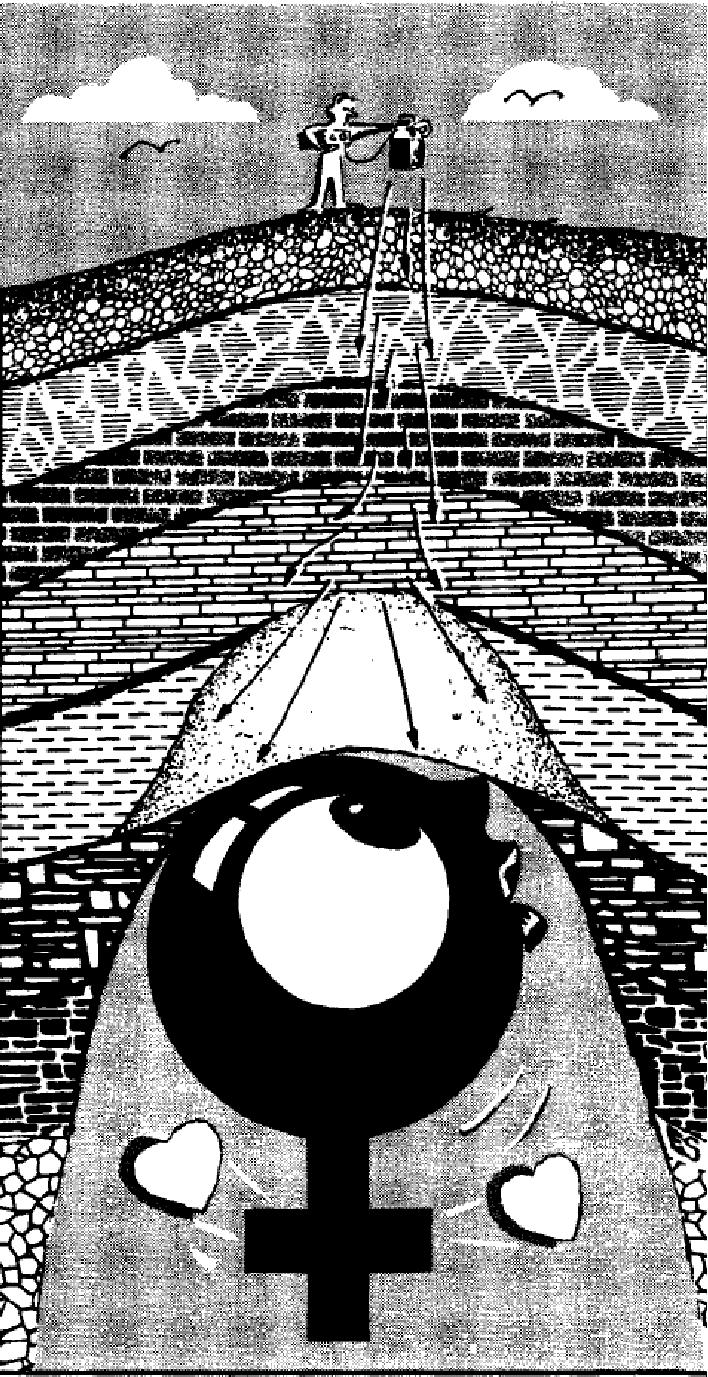
\includegraphics[height=\textheight]{Fig/magic}
\end{center}
\end{minipage}
\end{frame}

\begin{frame}
\MadLogo
\frametitle{Black Magic in Computational Science}

\quotebox{ 
Within the world of science, computation is now rightly seen as a
third vertex of a triangle complementing experiment and
theory. However, as it is now often practiced, one can make a good
case that computing is the {\color{blue}{last refuge of the scientific scoundrel}} [...] 
Where else in science can one get away with publishing observations
that are claimed to prove a theory or illustrate the success of a
technique without having to give a careful description of the methods
used, in sufficient detail that others can attempt to repeat the
experiment?}{Randall LeVeque}{ICM, 2006}

\end{frame}

\begin{frame}
\MadLogo
\frametitle{(Hale, 1984)}
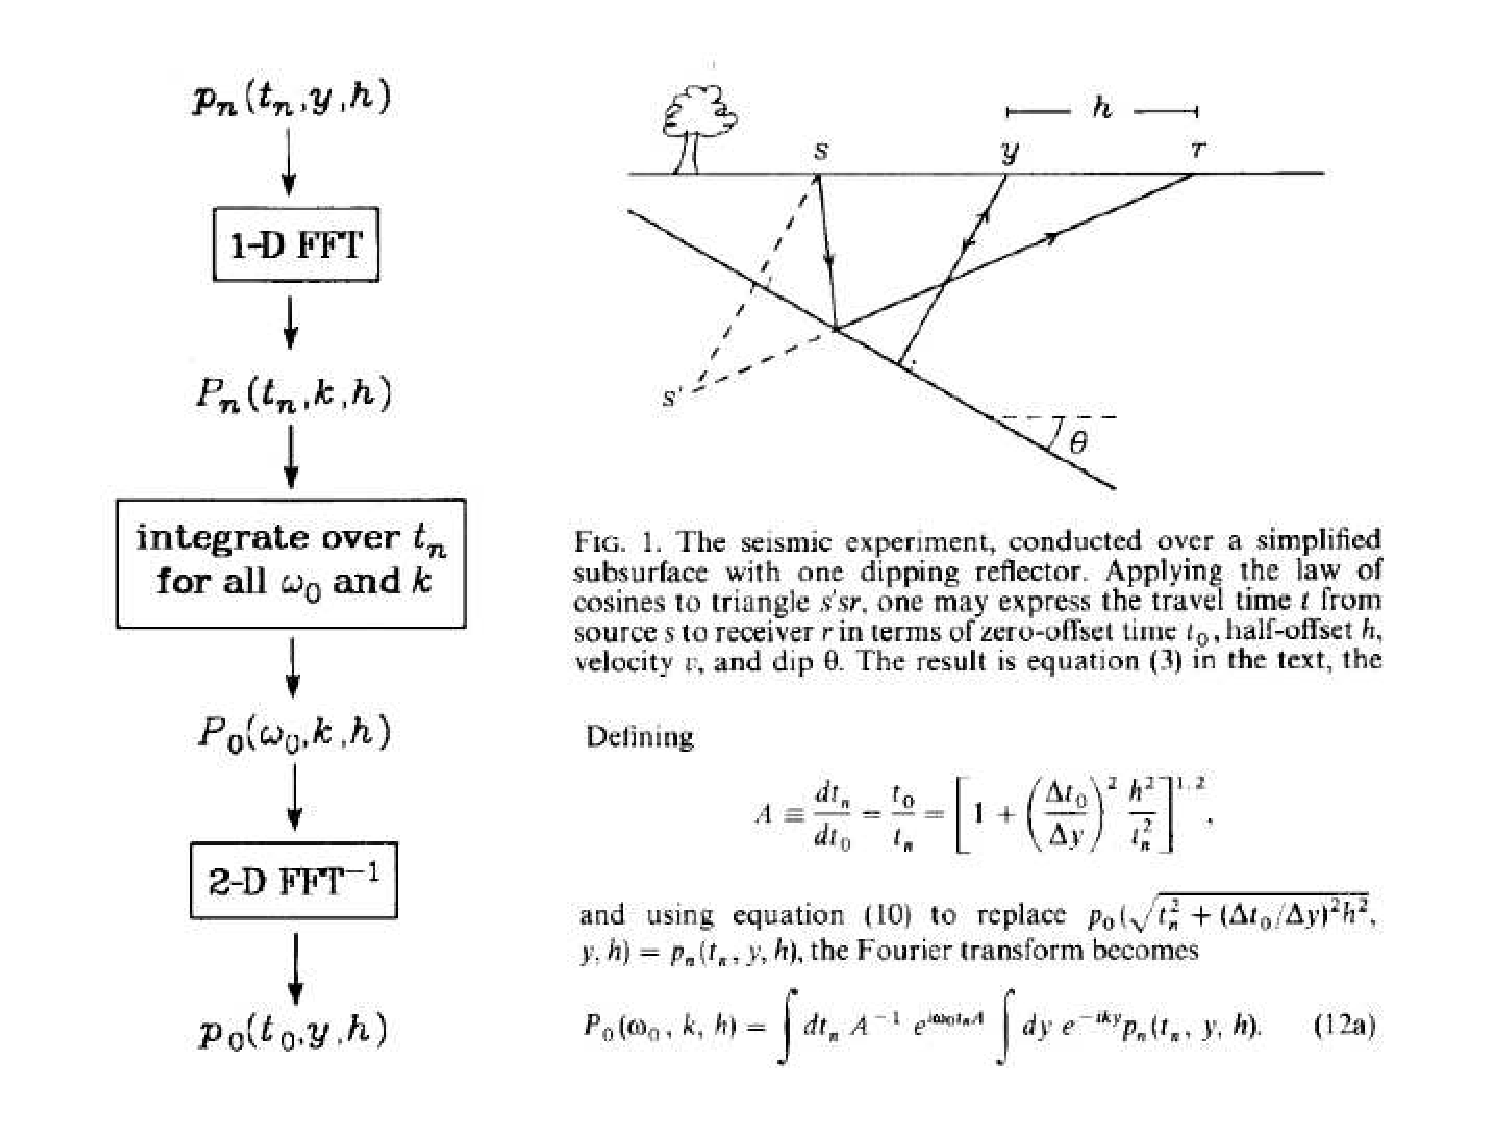
\includegraphics[height=0.8\textheight]{Fig/Hale1}
\end{frame}

\begin{frame}
\MadLogo
\frametitle{(Hale, 1984)}
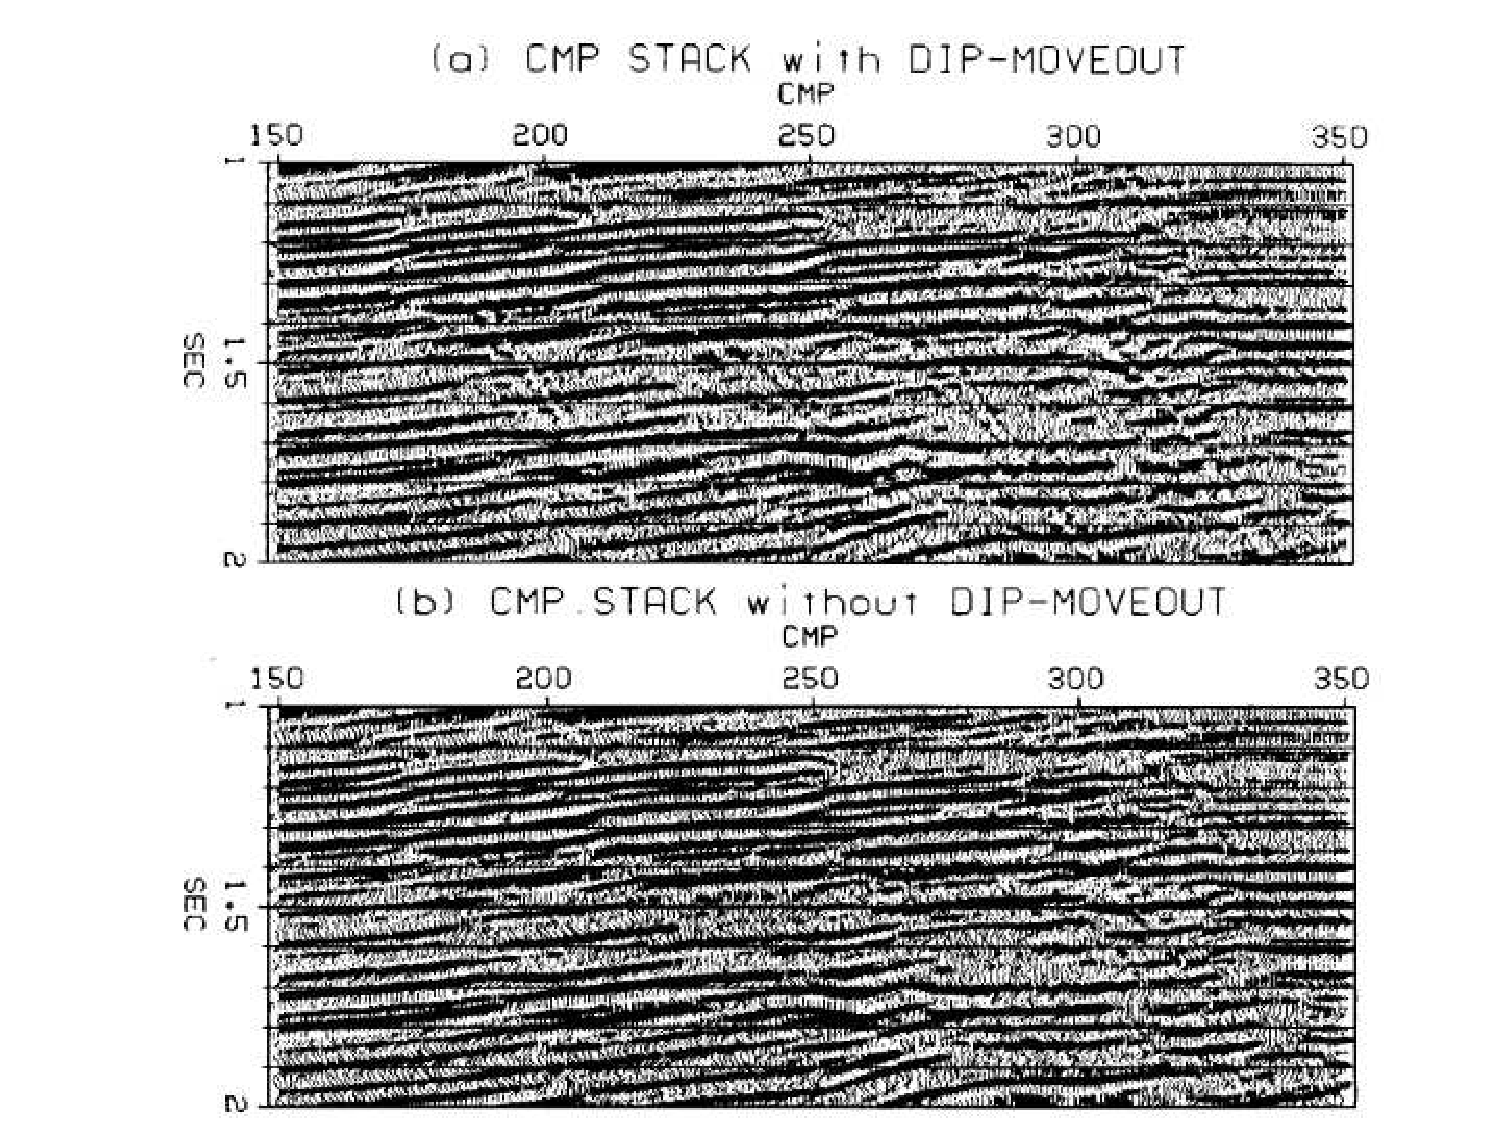
\includegraphics[height=0.8\textheight]{Fig/Hale2}
\end{frame}

\begin{frame}
\MadLogo
\frametitle{What is Science?}

\begin{center}
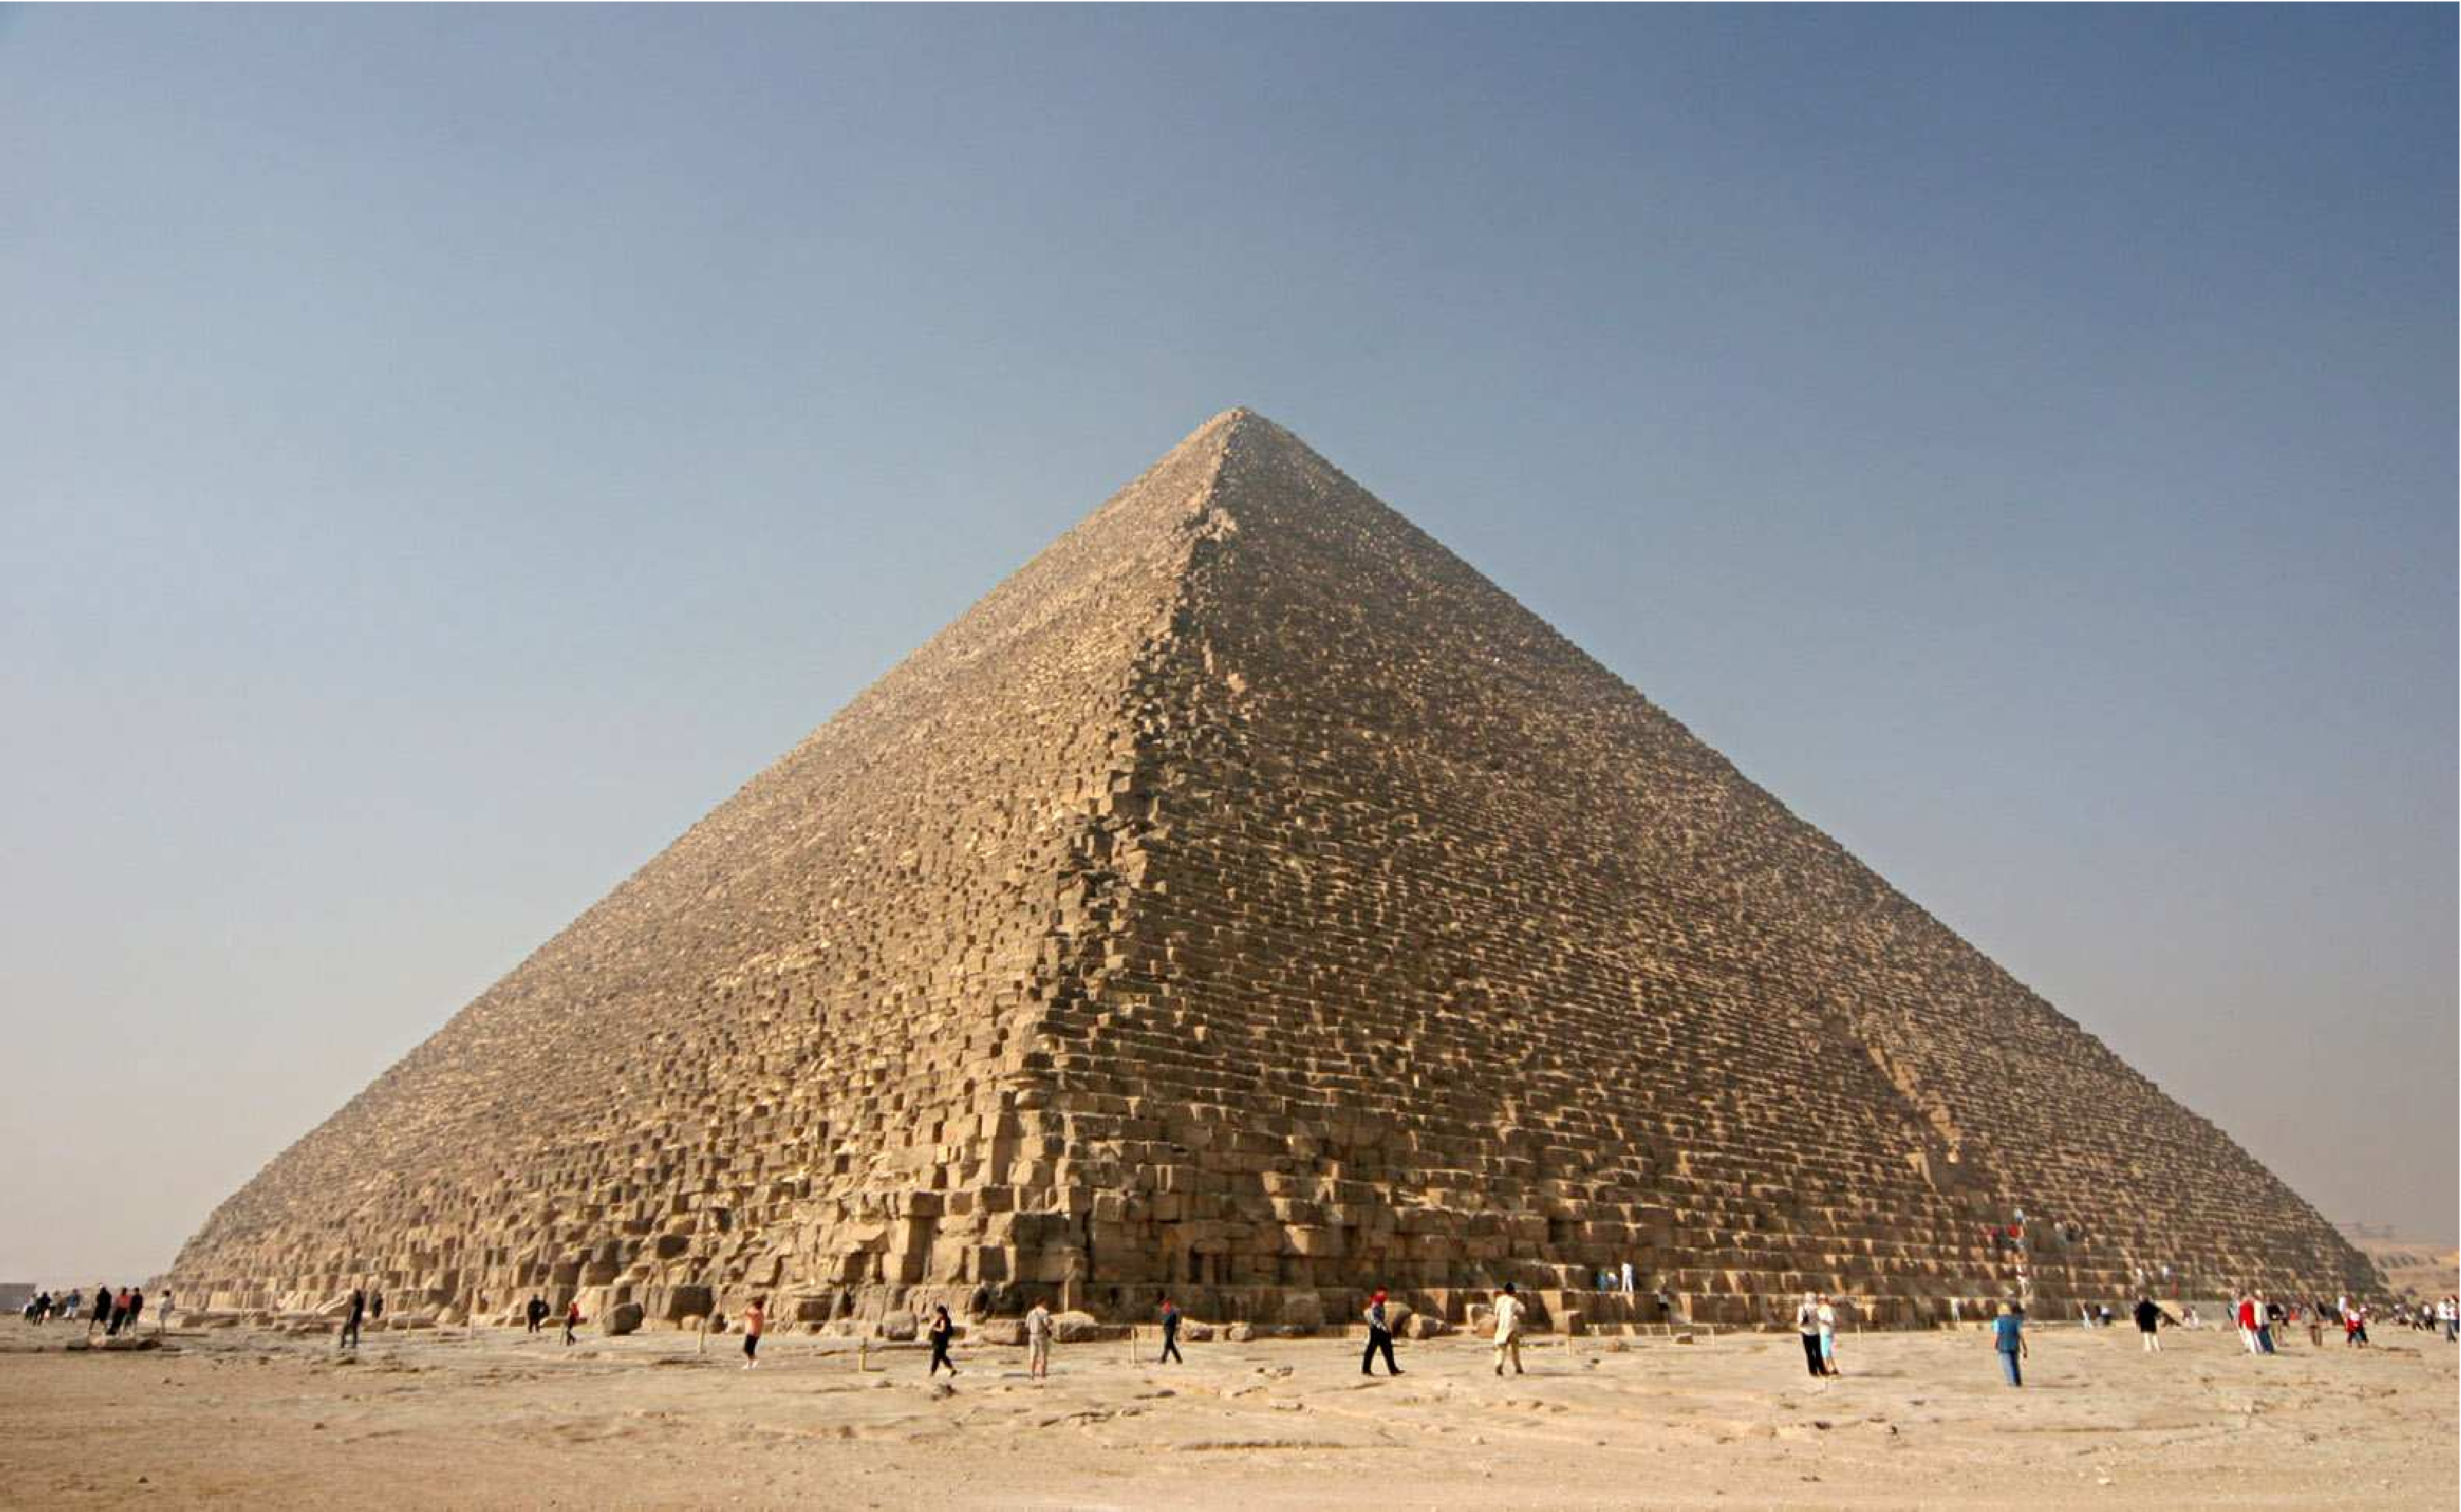
\includegraphics[height=0.8\textheight]{Fig/Kheops-Pyramid}
\end{center}
\end{frame}

\begin{frame}
\MadLogo
\frametitle{What is Science?}

\quotebox{{\Large \color{blue}{Science}} is the systematic enterprise of gathering knowledge about the universe and organizing and condensing that knowledge into testable laws and theories. The success and credibility of science are anchored in the willingness of scientists to {\Large \color{red}{independent testing and replication}} by other scientists. This requires the complete and {\Large \color{red}{open exchange of data, procedures and materials}}.}{American Physical Society}{What is science}
\end{frame}

\begin{frame}
\MadLogo
\frametitle{From Science to Open-Source Software}

\quotebox{{\Large \color{blue}{Abandoning the habit of secrecy}} in favor of process
  transparency and peer review was the crucial step by which alchemy
  became chemistry.  In the same way, it is beginning to appear that
  open-source development may signal the long-awaited maturation of
  software development as a discipline.}  {\\ Eric Raymond}{TAUP,
  2004}
\end{frame}

\begin{frame}
\MadLogo
\frametitle{What is Reproducible Research?}

\begin{itemize}
\item Attaching code and data to publications
\item Code requires continuous maintenance
\item Maintenance requires an open community
\end{itemize}

  \quotebox{
An article about computational science in a scientific publication is not the
scholarship itself, it is merely advertising of the scholarship. The actual scholarship
is the complete software development environment and the complete
set of instructions which generated the figures.}
{Jon Buckheit and David Donoho}{WaveLab, 1995}
\end{frame}

\begin{frame}
  \MadLogo
  \frametitle{Jon Claerbout's Story}

  {\flushright
  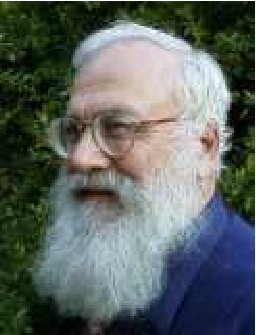
\includegraphics[height=0.2\textheight]{Fig/Claerbout}
  } 

  \begin{description}
  \item[1987] Sunview experience
  \begin{itemize}
  \item	Interactive programs are slavery
  \end{itemize}
  \item[1992] \LaTeX\ + \texttt{cake}
  \begin{itemize}
  \item Building books by a single command
  \end{itemize}
  \item[1990s] Ph.D. students
  \begin{itemize}
  \item \texttt{cake} to \texttt{make}, CD-Rom to WWW
  \end{itemize}
  \item[2001] Reproducible research paper in \emph{CiSE}
  \begin{itemize}
  \item {\color{blue}{The principal beneficiary is the author}}
  \end{itemize}
  \end{description}
\end{frame}

\begin{frame}
  \MadLogo
  \frametitle{Moving Forward}
  \begin{minipage}{0.25\textwidth}
  \begin{center}
  
\includegraphics[width=\textwidth]{Fig/CiSE}
  \vfill \ 
\end{center}
  \end{minipage} \hfill
   \begin{minipage}{0.65\textwidth}
  \begin{description}
    \item[ICASSP 2007] \ 
    \item[Berlin-6 2008] \
    \item[CiSE 2009] 
    \begin{itemize}
    \item Fomel \& Claerbout
    \item Donoho et al.
    \item LeVeque
    \item Ping \& Eckel
    \item Stodden
    \end{itemize}
    \item[IEEE Signal Processing Magazine 2009] 
    \begin{itemize}
    \item Vandewalle et al.
     \end{itemize}
     \item[\url{http://www.reproducibleresearch.net}] \ 
   \end{description}
  \end{minipage}
\end{frame}

\section{History of \textsc{Madagascar}}

\begin{frame}<beamer>
  \MadLogo
  \frametitle{Outline}
  \tableofcontents[currentsection]
\end{frame}

\begin{frame}
  \MadLogo
  \frametitle{Basic Information}

  \begin{itemize} 
  \item Started around 2003 
  \item Publicly available since June 12, 2006 
  \item Current version: 0.9.8 
  \item Vladimir Bashkardin, Jules Browaeys, Cody Brown, Maria Cameron, 
  Joseph Dellinger, Sergey Fomel, Gilles Hennenfent, Trevor Irons, Jim
  Jennings, Long Jin, Guochang Liu, Yang Liu, Doug McCowan, Henryk
  Modzelewski, Colin Russell, Paul Sava, Jeffrey Shragge, Xiaolei
  Song, Eduardo Filpo Silva, Ioan Vlad, Jia Yan
  \item	Jon Claerbout, Steve Cole, Dave Hale, Chuck Karish, Stewart Levin, Dave Nichols, Shuki Ronen
    \item \color{blue}{{\Large \bfseries \url{http://www.ahay.org/}}} 
    \end{itemize}
\end{frame}

\begin{frame}
  \MadLogo
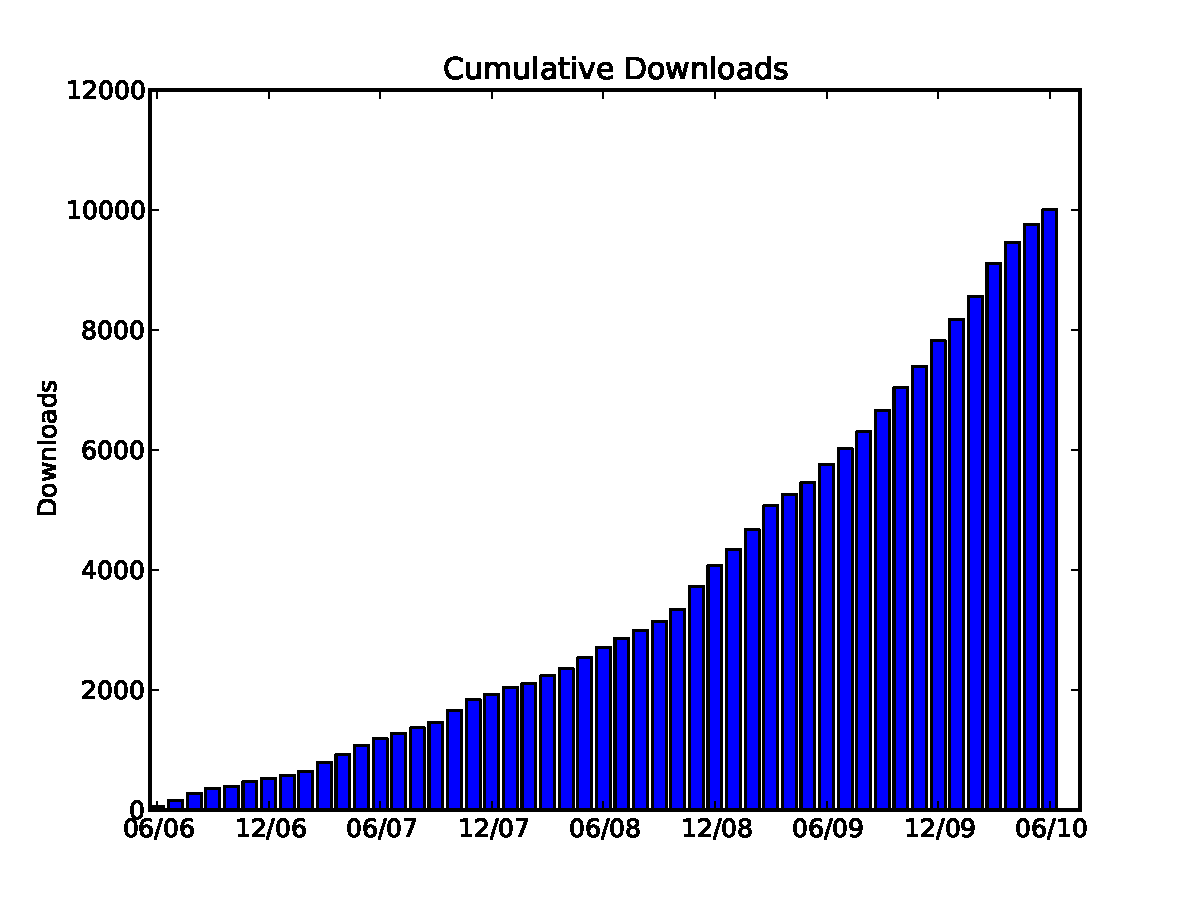
\includegraphics[width=\textwidth]{Pylab/Fig/downloads}  
\end{frame}

\begin{frame}
  \MadLogo
  \frametitle{Website Traffic: April 2009/April 2008}

\begin{center}
  \begin{tabular}{lr} 
\textbf{Twitter:} & 1,300\% \\
\textbf{\textsc{Madagascar}:} & 970\% \\
\textbf{Facebook:} & 220\% \\
\textbf{Google:} & 10\% \\
\textbf{Myspace:} & -10\%
  \end{tabular}
\end{center}
  
  \begin{itemize}
  \item	{\color{blue}{How Twitter Will Change the Way We Live}} 
  \item	 Steven Johnson, \emph{TIME}, June 5, 2009 
  \end{itemize}
\end{frame}

\begin{frame}
  \MadLogo
  \frametitle{Access Geography}
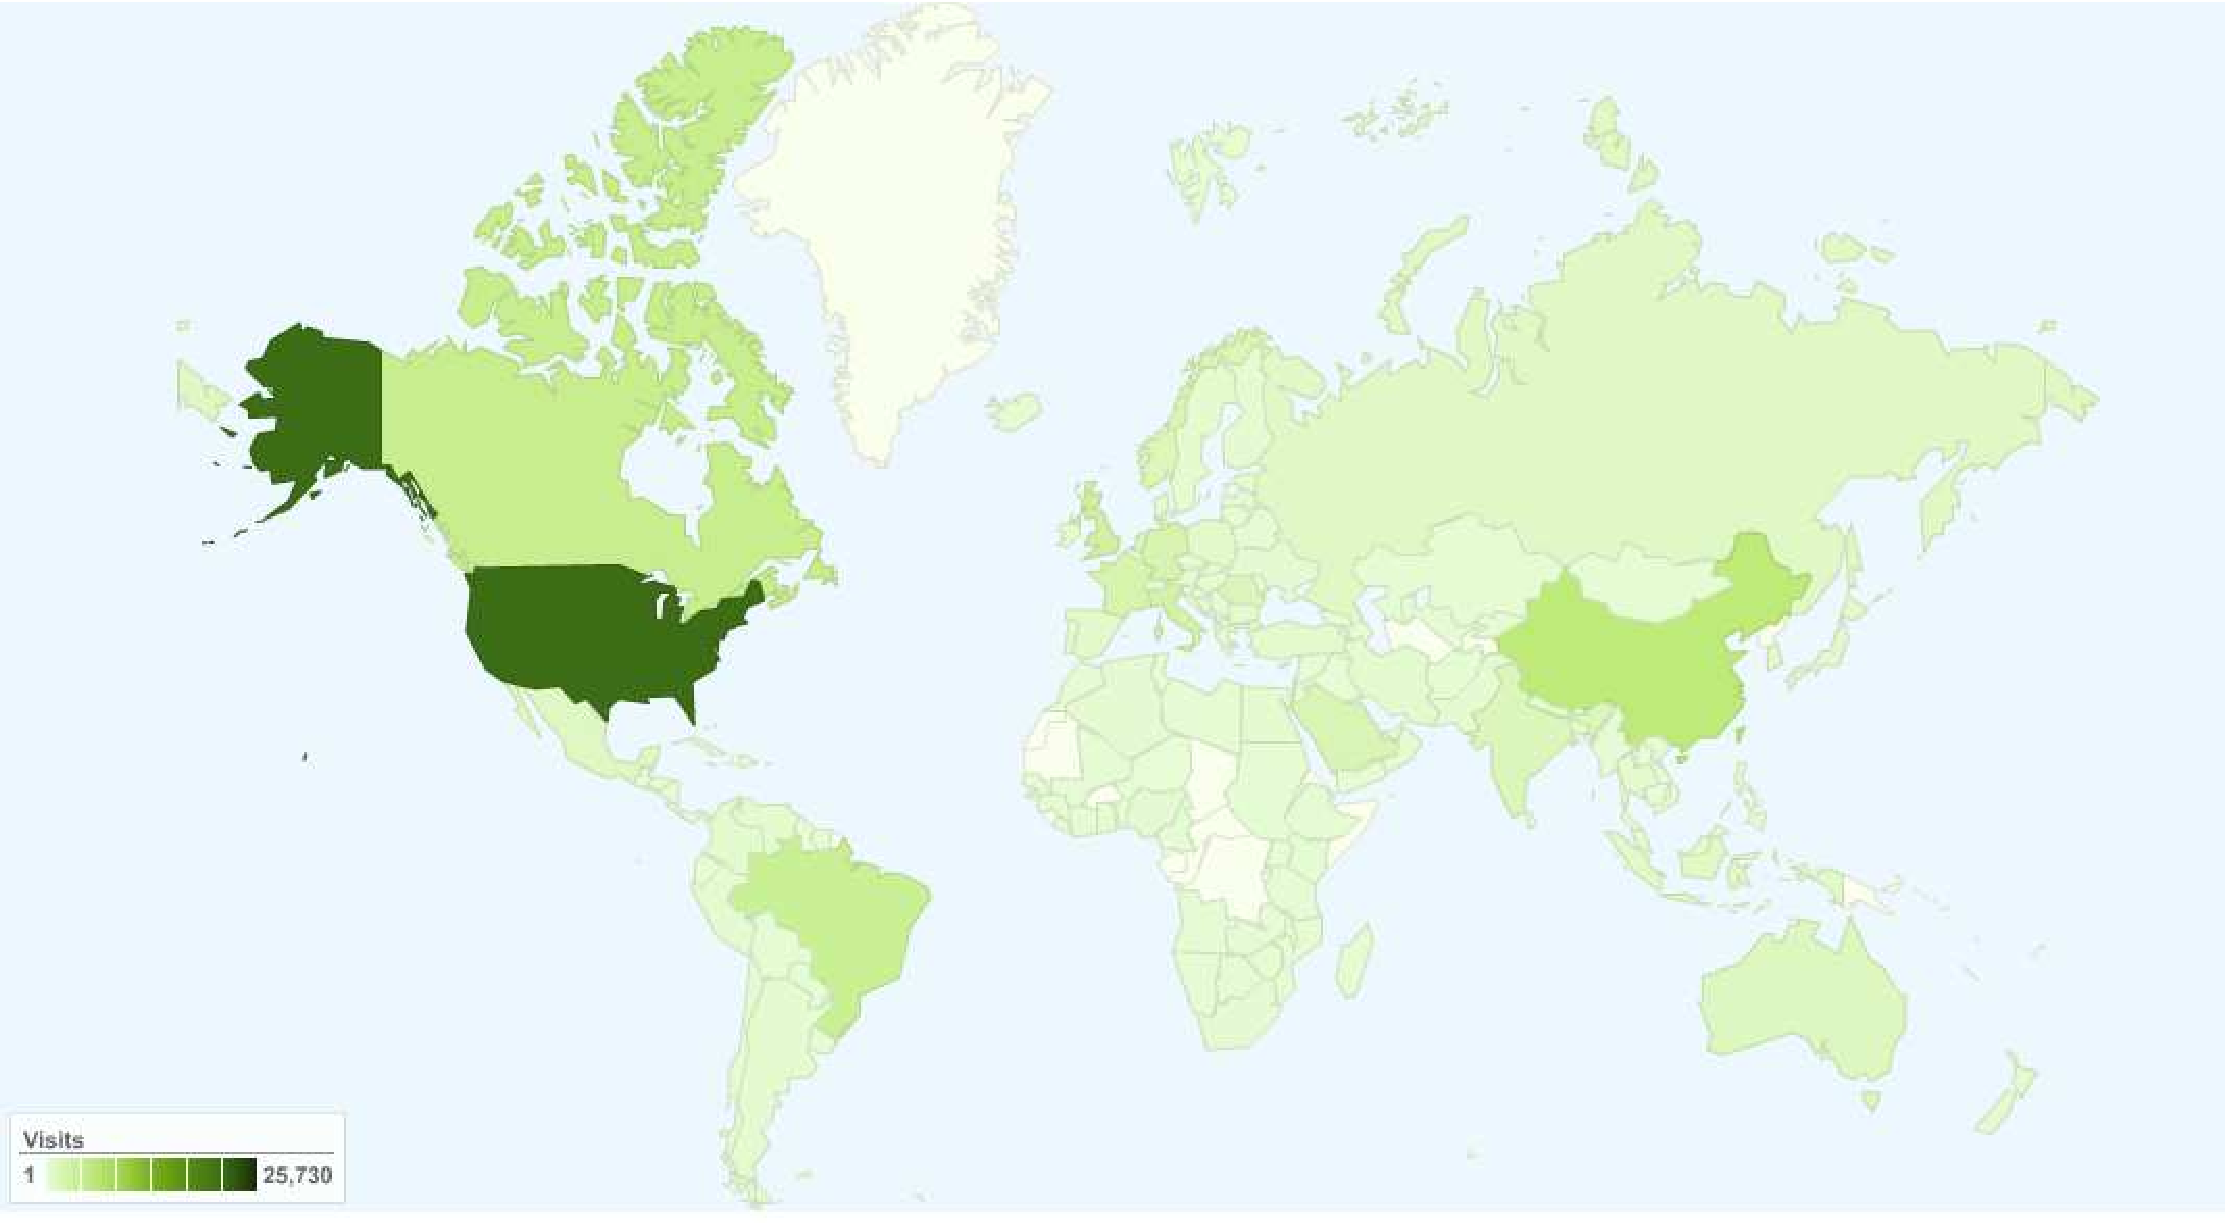
\includegraphics[width=\textwidth]{Fig/map}  
\end{frame}

\begin{frame}
  \MadLogo
  \frametitle{School and Workshop: Vancouver 2006}
  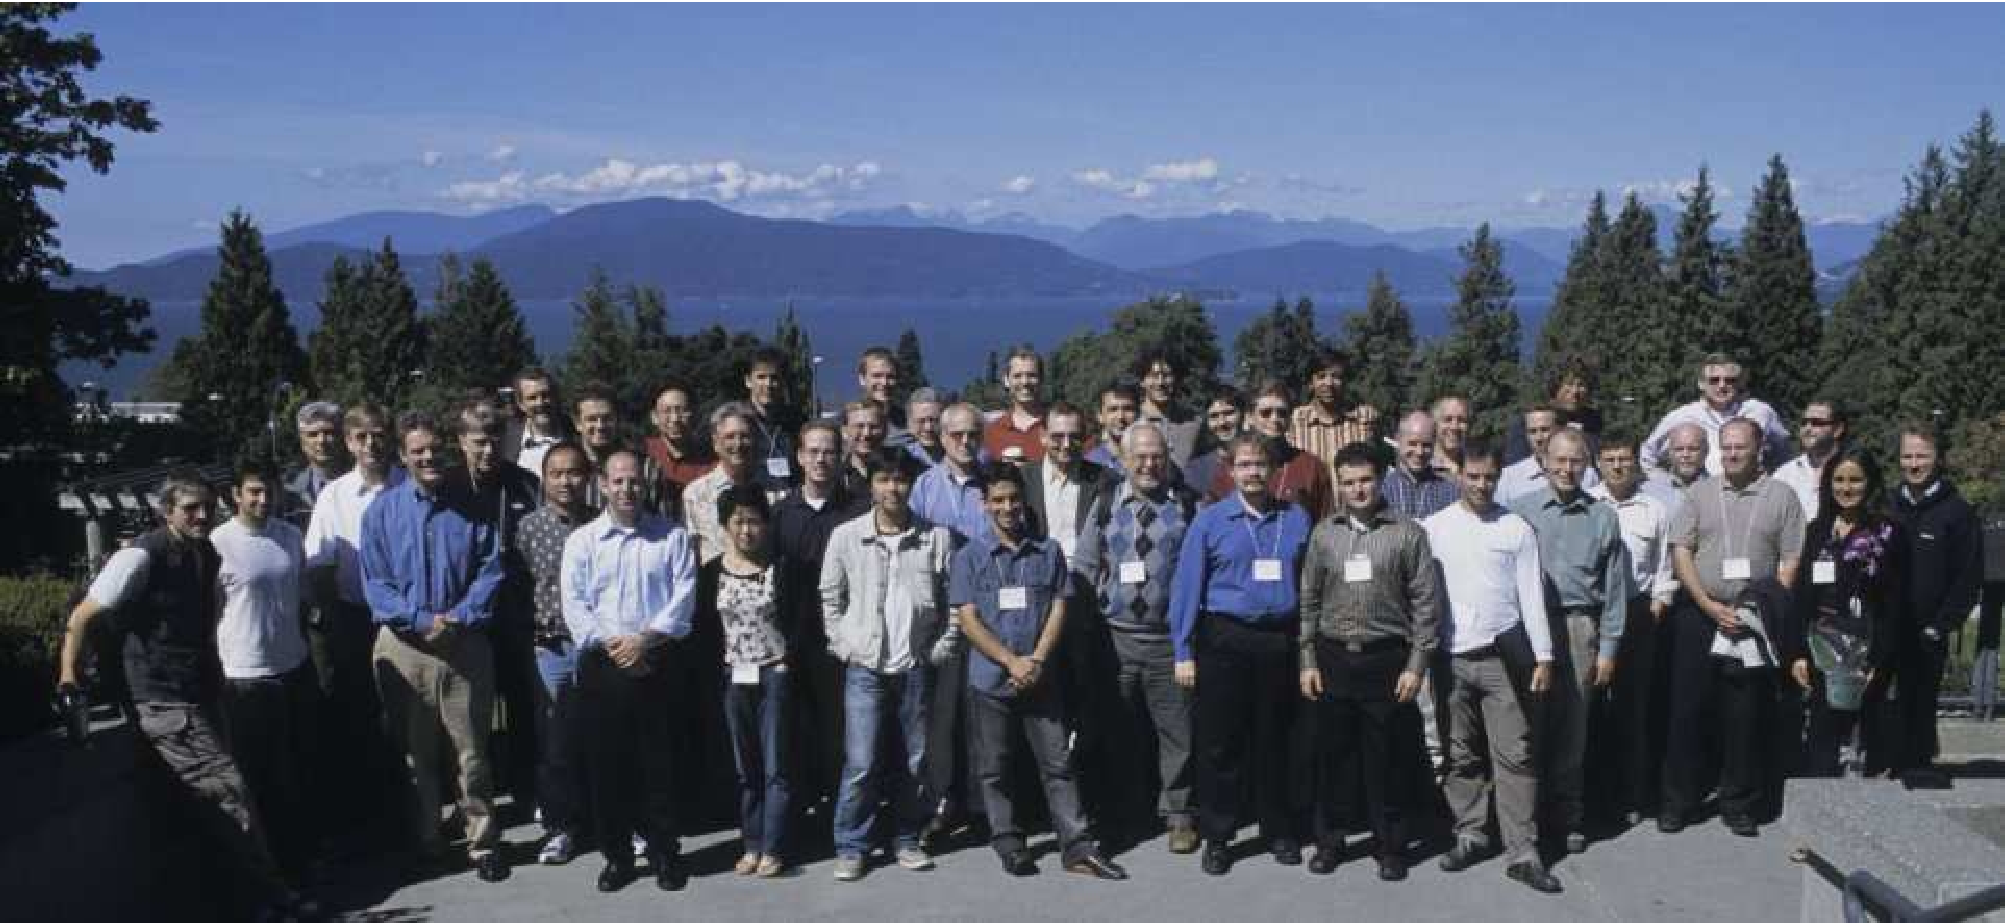
\includegraphics[width=\textwidth]{Fig/RSF2006}
\end{frame}

\begin{frame}
  \MadLogo
  \frametitle{School: Austin 2007}
  \begin{minipage}{0.45\textwidth} 
  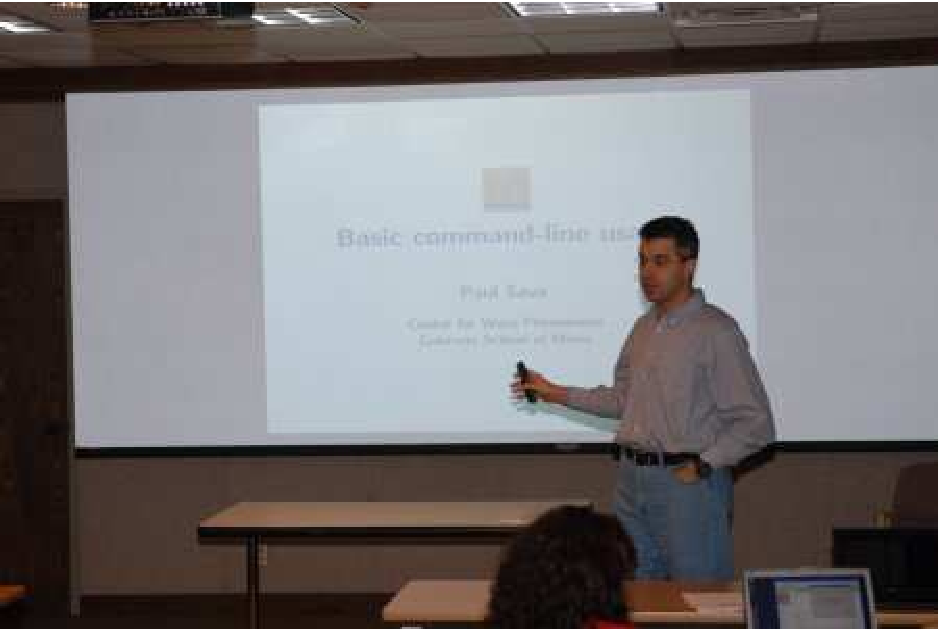
\includegraphics[width=\textwidth]{Fig/Paul}
   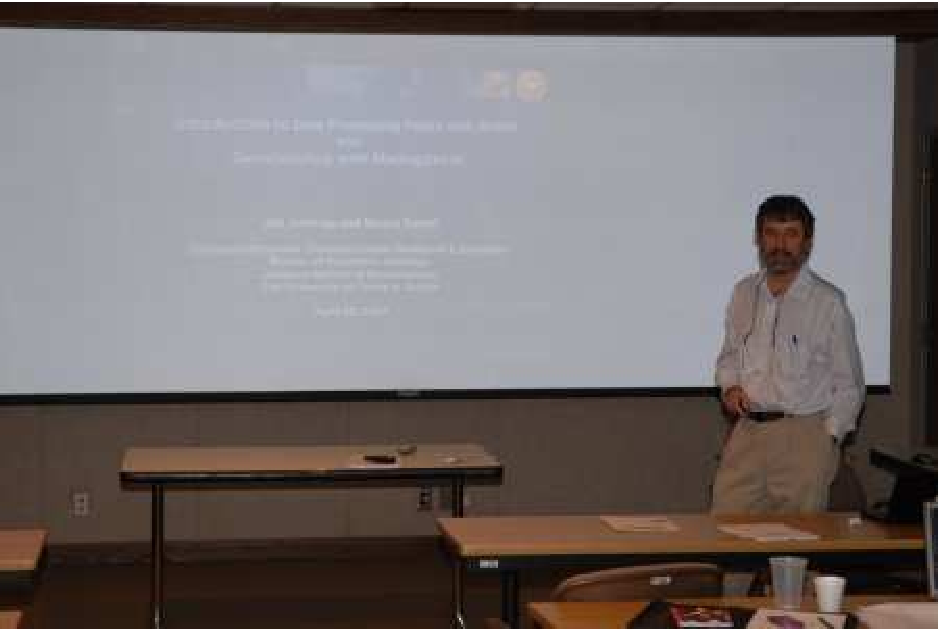
\includegraphics[width=\textwidth]{Fig/Jim}
  \end{minipage} \hfill
  \begin{minipage}{0.45\textwidth}
  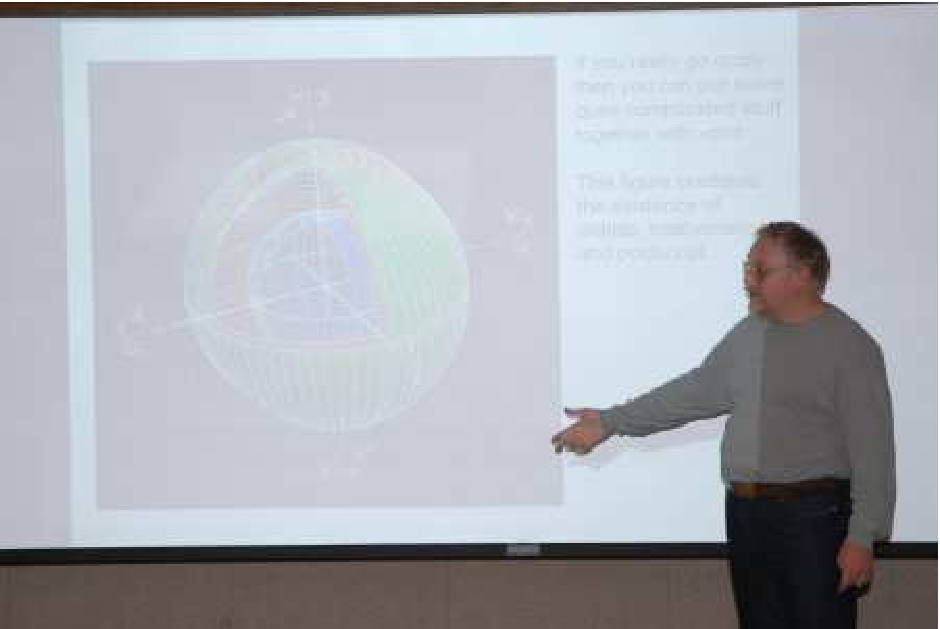
\includegraphics[width=\textwidth]{Fig/Joe}
   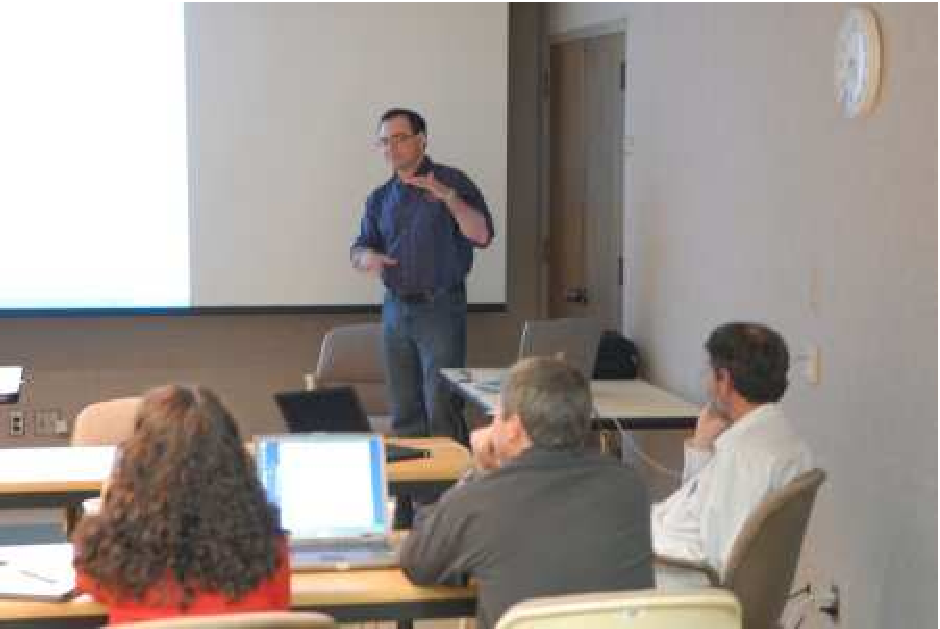
\includegraphics[width=\textwidth]{Fig/Sergey}
   \end{minipage}
\end{frame}

\begin{frame}
  \MadLogo
  \frametitle{Developer Workshop: Golden 2008}
  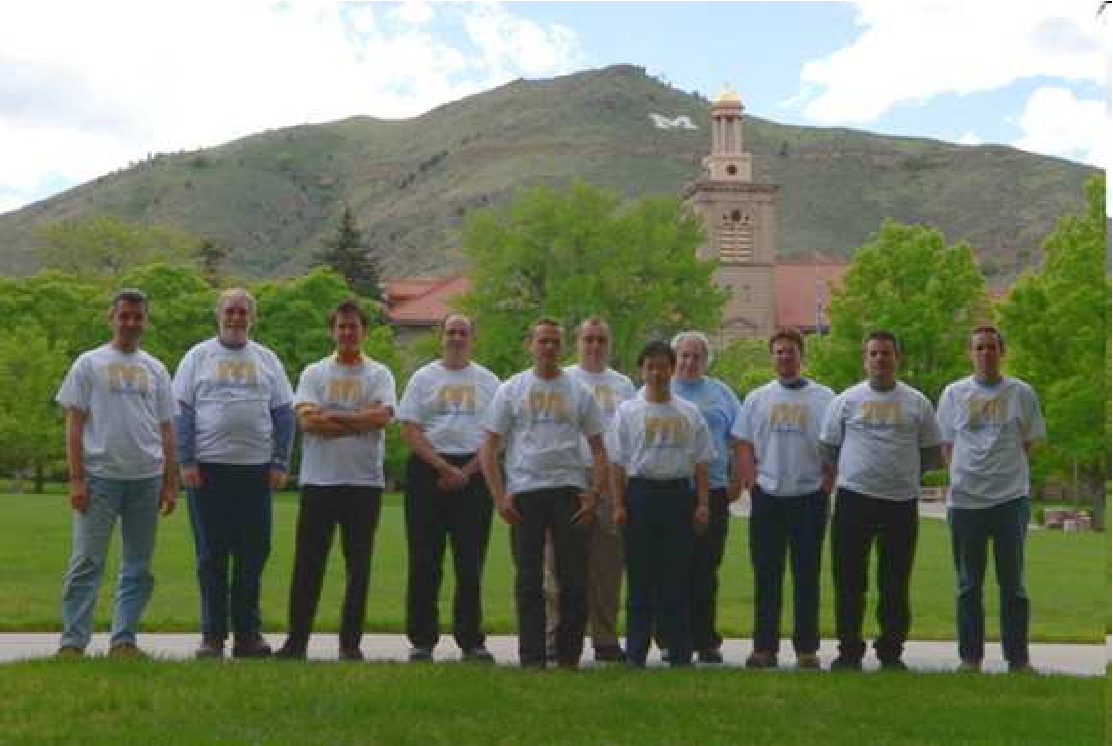
\includegraphics[height=0.7\textheight]{Fig/RSF2008}
\end{frame}

\section{\textsc{Madagascar} Components}

\begin{frame}<beamer>
  \MadLogo
  \frametitle{Outline}
  \tableofcontents[currentsection]
\end{frame}

\begin{frame}
  \MadLogo

  \frametitle{One Week Technology Transfer}
  \begin{tabular}{rl}
  \textbf{\color{blue}{Monday:}} & Get an idea \\
  \textbf{\color{blue}{Tuesday:}} & Implement it \\
  \textbf{\color{blue}{Wednesday:}} & Test it \\
  \textbf{\color{blue}{Thursday:}} & Communicate it \\
  \textbf{\color{blue}{Friday:}} & Apply it in practice
  \end{tabular}
\end{frame}

\begin{frame}
  \MadLogo
  \frametitle{\textsc{Madagascar} Components}

    \begin{description}
    \item[Tuesday:] Implement it
      \begin{itemize}
      \item Main programs (C, C++, Fortran, etc)
      \item \href{http://www.reproducibility.org/RSF/}{600 modules}
      \end{itemize}
    \item[Wednesday:] Test it
      \begin{itemize}
      \item Data processing flows (Python/SCons)
      \item 300 scripts $\rightarrow$ 2,400 figures
      \end{itemize}
    \item[Thursday:] Communicate it
      \begin{itemize}
      \item Books and papers (\LaTeX/SCons)
      \item \href{http://www.ahay.org/Reproducible_Documents}{100 papers}
      \end{itemize}
    \end{description}
\end{frame}

\begin{frame}
  \MadLogo
  \frametitle{\textsc{Madagascar} Objectives}

  \begin{itemize}
  \item To make computational research efficient
  \item To make it easy to share computational results
  \item To maintain an open community
  \end{itemize}
\end{frame}

\begin{frame}
  \MadLogo
  \frametitle{\textsc{Madagascar} Design Principle}

  \begin{itemize}
  \item Document computational experiments and use them in the future as regression {\color{blue}{tests}}
  \item {\color{blue}{Reproducible research}}
  \item Test-driven development
  \item YAGNI (You Ain't Gonna Need It)
  \end{itemize}

  \quotebox{Always implement things when you actually need them, never when you just foresee that you need them.}{Ron Jeffries}{YAGNI}  
\end{frame}

%\begin{frame}
%  \MadLogo
%  \frametitle{RSF file format}
%  \begin{itemize}
%  \item	Universal \href{http://www.ahay.org/Format}{data file format}
%  \begin{itemize}
%  \item mostly compatible with SEPlib
%  \end{itemize}
%  \item	Data separated from text headers
%  \item Conceptually $N$-D hypercubes
%  \item Multiple files for irregular geometries
%  \end{itemize}
%\quotebox{If you feel an urge to design a complex binary file format, or a complex binary application protocol, 
%          it is generally wise to lie down until the feeling passes.}{Eric Raymond}{TAUP}
%\end{frame}

\begin{frame}
\frametitle{Conclusions}
\begin{center}
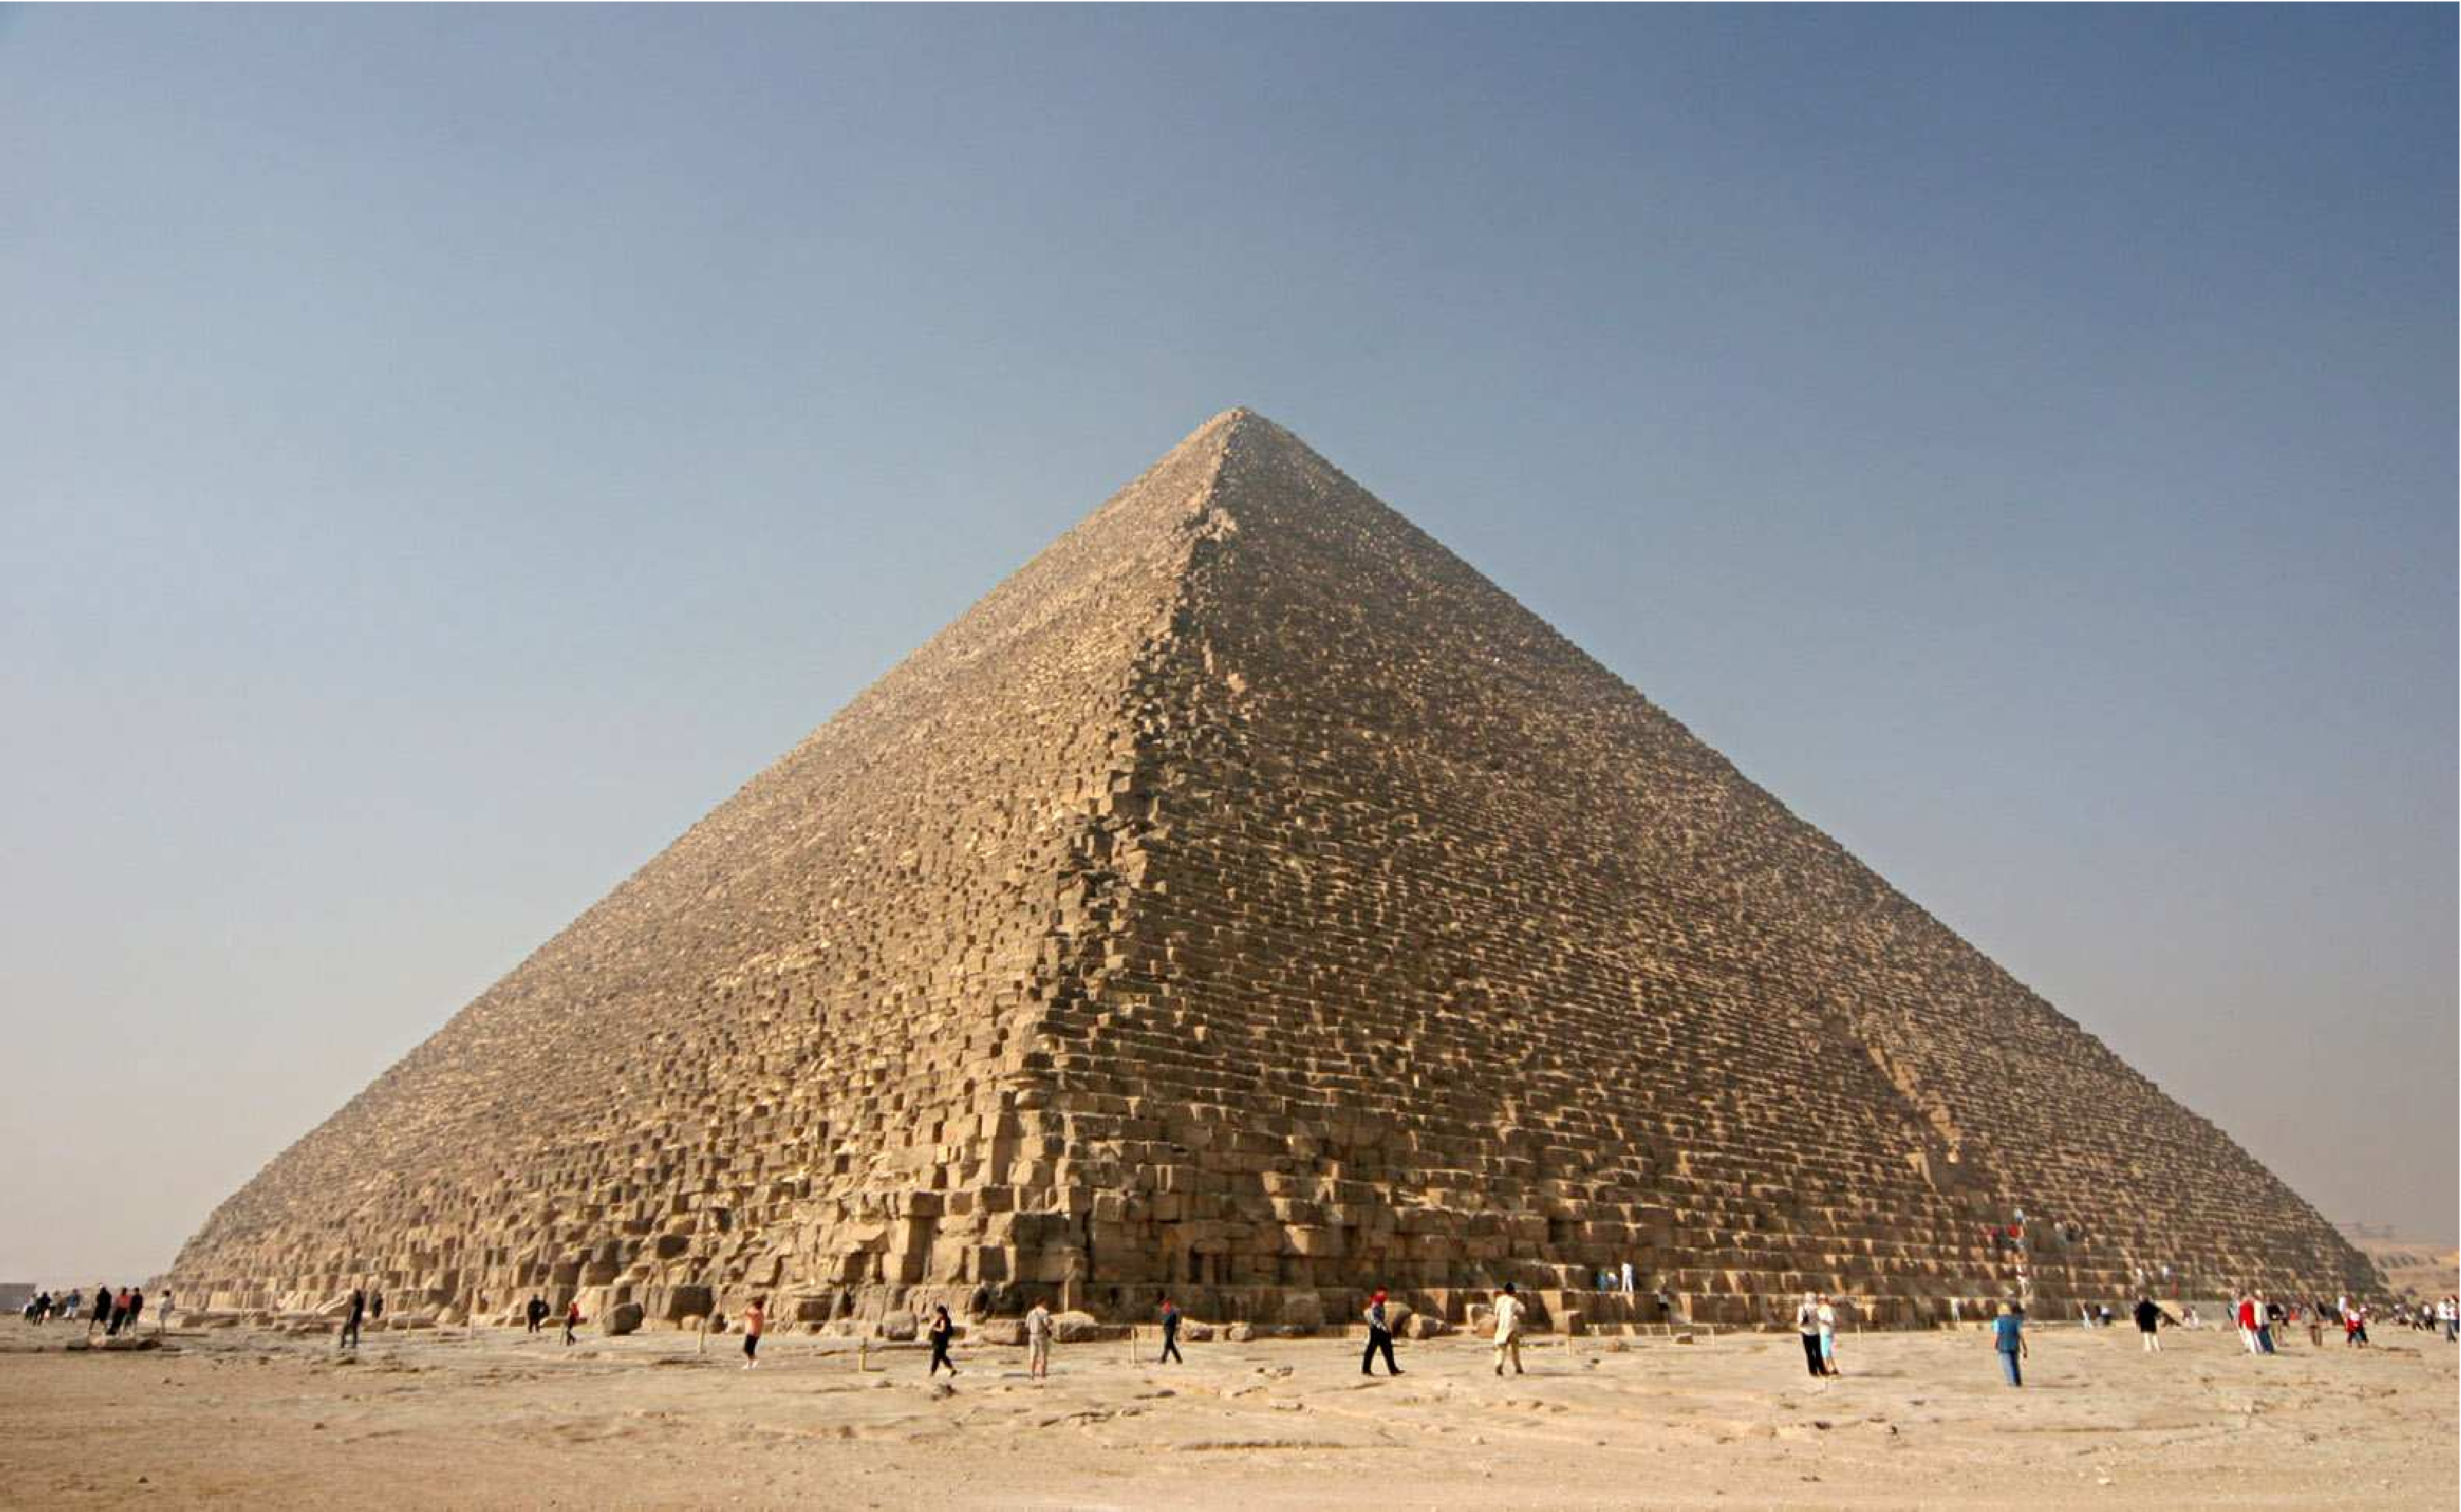
\includegraphics[height=0.6\textheight]{Fig/Kheops-Pyramid}
\end{center}

  \begin{itemize}
  \item Reproducible computational experiments
  \item {\color{blue}{\textbf{\url{http://www.ahay.org/}}}}
  \item Help is needed
  \end{itemize}
\end{frame}
